\documentclass{article}
\usepackage{graphicx}
\begin{document}

\begin{center}
\Huge Andreas Landgrebe
\\
Pledge:
\\
Computer Science 440
\\
Laboratory Assignment One
\\
Customizing and Using the Z Shell
\\


\includegraphics[width=5in]{images/zsh.png}
\end{center}



\newpage
\begin{enumerate}
\item Using screenshots and concrete examples, a description of the key features provided by zsh.
\\
\\
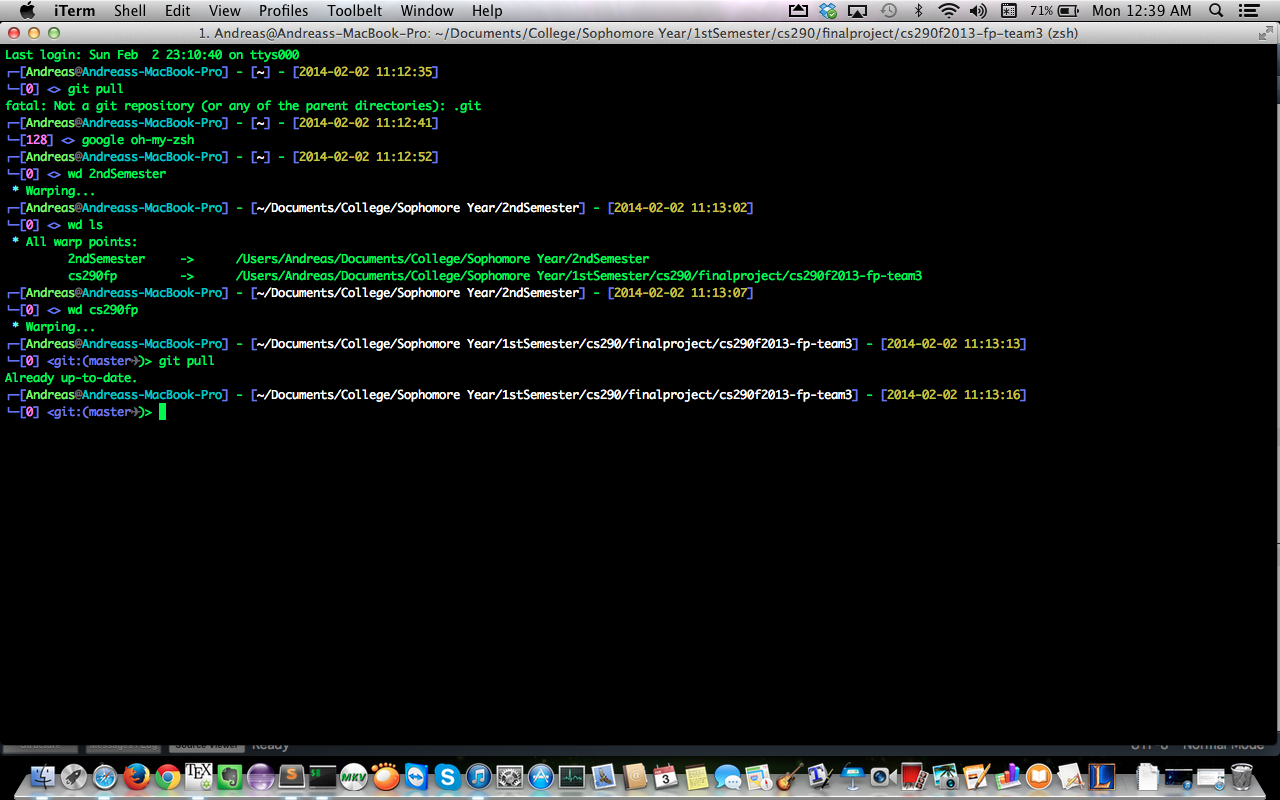
\includegraphics[width=5in]{images/prompt2.png}
\\
\\
Some of the key features that zsh provides is easier customization of the features and display of a terminal prompt. Some key features that zsh provides is being able to change the themes to make the prompt look nice when in use. Another key feature that zsh provides is all of the available plug-ins. One of the key plugins that I found to be useful is the web-search to be able to do a google search or use another search engine to look something up.
\\
\item A commentary on the features that zsh provides that your previous shell did not
\\
There are several features that zsh provides that my previous shell did not. With this zsh shell installed, I am able to cusotmize the display of the shell much easier. By changing the themes in the ~/.zsh file, I am able to customize the display on the terminal in any fashion. For example, in the themes settings that I have specified, I am able to display the date and time of a particular moment. Another feature that zsh provides that my previous shell did not was being able to add specific plugins to be able to perform specific commands. One of the commands that I can run now that I coud not run before was being able to write the command google in the terminal and be able to look up what I have specified to look up in google.
\\
\item A tutorial that explains how to download, install and configure oh-my-ssh, including how to:
\begin{enumerate}
\item Install the oh-my-zsh community driven framework
\\
In order to install the oh-my zsh community driven framework, there are a few ways to do so. One of the ways to do so is by using wget commands by pressing the following command into the terminal:
\\
\\
wget --no-check-certificate https://raw.github.com/robbyrussell/oh-my-zsh/master/tools/install.sh -O -
\\
\\
The other way to do this is by cloning the repository the manual way which is the way that I used to install the oh-my-zsh framework. The following command is what I had used:
\\
\\
git clone git://github.com/robbyrussell/oh-my-zsh.git ~/.oh-my-zsh
\\
\\
one of the previous 2 commands would have worked in order to install the oh-my-zsh framework
\\
\item Change the display of the zsh prompt (e.g., show the user name and host name)
\\
In order to change the display of the zsh prompt, when would need to open up ~/.zsh from the command line to change the theme of the available configuration. Once you are successful in opening this file in a text editor, you will see a file opened. In this file, on the 8th line, this is the line you would change in order to change the theme. There are several available themes you can choose from the following website:
\\
\\
https://github.com/robbyrussell/oh-my-zsh/wiki/themes
\\
\\
From this website, you will see several different themes that you can choose from. You can only choose 1 theme to use at a particular time but you can use as many plugins as you want.  
\item Commentary on how to install, configure, and use the following zsh plugins
\\
\begin{enumerate}
\item git
\\
In order to install the git plug-in for the zsh shell, you would need to open the \~/.zschrc through any of the available text editors (personally I used Sublime Text so I ran the command: subl \~/.zshrc). After this file has been opened in a text editor, you will now be able to choose which plug-ins you would like to install for your zsh shell. There are many different plug-ins, a list of plugins is availalbe on this website:
\\
\\
https://github.com/robbyrussell/oh-my-zsh/wiki/Plugins
\\
\\
After you have found which plug-in to install for the zsh, on line 48 of this file, there should be a line to start with the words plugins. On this line, in the brackets that are already there, one can install any of the availalbe plug-ins for the zsh. In order to install the git plug-in you would type to words git in the brackets where it says plugins. You are available to install as many plug-ins as you would like, the only that you would need to do is that for each different plugin, it needs to be made sure that each plugin is seperated by a space.
\\
For this case, the git plug-in is a plug-in that will allow you to pull and push changes to a specific verison control repository. This feature is important for any computer scientist. There is not one computer scientist that comes to mind that does not use version control. Using version control repostiories is important in order to do future laboratory assignment when you are asked to work in a group. Using git commands will allow you to retrieve information that has been done to a repository when changes have been applied, it will also allow you to save information when you have worked on a project and is available to the rest of the group that has been given access to make changes to the repository. The git commands also has many different features to be used in order to complete a specific task as a group.
\\
\\
\item web-search
\\
In order to install the web-search plug-in to the zsh shell, you would need to follow the same instructions you would use to install the git plugins but instead of the writing git in the brackets after it stays plugins, you would write web-search. You can install as many plug-ins as you want onto this zsh. In order to use the web-search plug-in, you can write the following in the terminal:
\\
google oh-my-zsh
\\
Once the web-search plugin has been install correctly, after this command has been run, your default browser will be opened and it will search on google oh-my-zsh. After the phrase google has been run in the terminal, you can type in anything to search on google. The oh-my-zsh was just an example.
\\
\item wd
\\
In order to install the wd plugin for zsh, you would need to follow the directions that are above by going into the \~./zschrc file by using a text-editor and add the plugins that you would like to install. In this case, if you would like to install the wd command, you would need to write wd in the brackets after the plugin. The wd plug-in will allow you to warp to a specific directory that has already been specific and the terminal will go to the specified directory already. This is a much more efficient way to change to directory than to use the command cd to change to each different directory. In order to configure this plug-in, you would need to go to the directory that you would want to be able to warp to. After this is done, you would want to write the command wd add. After the wd add command is type, you would need to specify a name of the specific directory that you would like to warp to. You can do this for as many directories as long as you do not give them the same names. If you would like to change a saved directory in the wd, you can choose the command wd add! to overwrite the saved directory or you could use the command wd rm, and the name of the saved directory to remove the saved directorty. 
\\
\item z
\\
In order to install this plug-in you would follow the same process as the past plugins and write z into plugins in the brackets and leave a space betwen the diferent plugins that have been installed. The z plugins will allow you to see the most commonly used directories. After a learning phase for z, the plugin can take to the most recent directory. There are many different options that can be shown using the z plugin by visiting the addressed specified here:
\\
https://github.com/robbyrussell/oh-my-zsh/tree/master/plugins/z
\\
\item zsh-syntax-highlighting
\\
In order to install the zsh-syntax highlighting, it is similar to how to install the other plugins but it is a little bit diferent. In order to install this plugin, you need to put source this script at the end of the plugin line of the \~./zshrc file. This plug-in acts similar to the fish shell for syntax highlighting. It is similar to the features of zsh when it comes to syntax highlighting.
\end{enumerate}
\item Set zsh as the default shell for your Ubuntu workstation
\\
In order to set zsh as the default shell there is a specific command to run through the terminal. I was working on my MacBook Pro so I was not wokrin on my Ubuntu workstation for this laboratory assignment. I decided on my own personal computer so I do not need to worry about having sudo or administrative access or anything of this nature. I also decided to make this decision because several of the commands that are available for the Ubuntu workstation are similar if not the same commands that can be run through the mac os x terminal. In order for me to use zsh as my default shell, I ran the command 
\\
cp ~/.oh-my-zsh/templates/zshrc.zsh-template ~/.zshrc
\\
This command this create a new zsh config by copying the zsh template. After this I ran the command,
\\
chsh -s /bin/zsh
\\
this command will create zsh to be the default shell and after you restart the terminal, the shell that will open up is zsh and not bash.
\end{enumerate}
\item A screenshot showing the final configuration of your zsh prompt in all relevant contexts
\\
Here is my final terminal prompt (I am using the rkj-repos theme and I will installed all of the plugins that were specified)
\begin{center}

\includegraphics[width=5in]{images/zsh.png}
\end{center}
\item A description of the challenges that you encountered when customizing and using zsh
\\
Some of the challenges that I had encountered when I was setting up zsh was being able to change the themes and the install the plugins. When I was trying to open up the \~./zsh, I had difficulty in opening a text editor to change the settings of the zsh. In order to do so, I had install a command on my terminal to be able to open a text editor like Sublime Text in order to change the settings to the specifications that I wanted. After I figured out how to open up a text editor to change the settings of the zsh, another difficulty that I had was being able to figure out what the zsh-syntax-highlighting was meant to do. After further researching the features that this plug-in has, all of my difficulties were gone.


\end{enumerate}
\end{document}